\documentclass[twocolumn]{el-author}

%\usepackage[...]{...}      This has been commented out as we are not using any additional packages here.  On the whole, they should be unnecessary.
\newcommand{\hH}{\hat{H}}
\newcommand{\D}{^\dagger}
\newcommand{\ua}{\uparrow}
\newcommand{\nc}{\newcommand}
\nc{\da}{\downarrow} \nc{\hc}{\hat{c}} \nc{\hS}{\hat{S}}
\nc{\bra}{\langle} \nc{\ket}{\rangle} \nc{\eq}{equation (\ref}
\nc{\h}{\hat} \nc{\hT}{\h{T}}\nc{\be}{\begin{eqnarray}}
\nc{\ee}{\end{eqnarray}}\nc{\rd}{\textrm{d}}\nc{\e}{eqnarray}\nc{\hR}{\hat{R}}\nc{\Tr}{\mathrm{Tr}}
\nc{\tS}{\tilde{S}}\nc{\tr}{\mathrm{tr}}\nc{\8}{\infty}\nc{\lgs}{\bra\ua,\phi|}\nc{\rgs}{|\ua,\phi\ket}
\nc{\hU}{\hat{U}}\nc{\lfs}{\bra\phi|}\nc{\rfs}{|\phi\ket}\nc{\hZ}{\hat{Z}}\nc{\hd}{\hat{d}}\nc{\mD}{\mathcal{D}}
\nc{\bd}{\bar{d}}\nc{\bc}{\bar{c}}\nc{\mc}{\mathcal}\nc{\ea}{eqnarray}\nc{\mG}{\mathcal{G}}\nc{\bce}{\begin{center}}
	\nc{\ece}{\end{center}}
\date{12th December 2011}
\begin{document}
	
	\title{OPPORTUNISTIC SPECTRUM ACCESS  WITH SENSING ERROR IN DISTRIBUTED  COGNITIVE
		RADIO NETWORKS}
	
	\author{Author 1 ,Author 2}
	
	\abstract{Spectrum access strategy is critical to realize cognitive radio. Taking in consideration the hardware limitations, channel dynamics and spectrum sensing error, we propose a dynamic spectrum access scheme for Decentralized Cognitive Radio (CR) networks. The main objective is to make efficient decisions on which channels to sense and access, that ensure maximization of the throughput of the cognitive user based on the partially observable Markov decision process model. This paper addresses spectrum sensing and channel selection strategy under imperfect spectrum sensing, and proposes opportunistic spectrum access scheme for the perfect and the imperfect spectrum sensing respectively. Simulation results show that under proposed scheme the Secondary Users (SU) can achieve superior performance in secondary network throughput and overall spectrum.}
	
	\maketitle
	
	\section{Introduction}
	Radio (CR) technology introduces challenges that did not exist in the static channel allocation networks. One of these challenges is the time varying availability of the spectrum bands which requires sophisticated algorithm at the secondary users to sense the spectrum\cite{AhmedGaniAbolfazliEtAl2016,Lunden2015}. In other words, the secondary users (SUs) have to continuously sense the whole spectrum which is energy inefficient, requires complex hardware, and then degrades the performance of the CR network.
	In this work, a channel access algorithm is proposed based on the Partially Observable Markov Decision Process POMDP channel model in which the SU uses the historical sensing information to estimate the condition or state of the primary channels. Accordingly, in the proposed algorithm the CR network is adapted based on the changes in the behavior of the primary network. Each SU computes the availability of the primary channel using the estimated channel states. Whenever the SU has data to transmit, it chooses a subset of the channels with the highest probability of being available to sense and thus it spends small time in sensing the channels. Therefore, the overhead time is reduced resulting in increasing the network throughput.
%	\section{Primary Network}
%	
%	\begin{figure}[h]
%		\centering
%		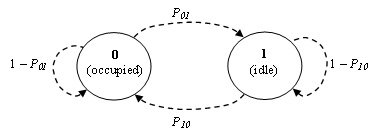
\includegraphics[width=0.7\columnwidth]{./pomdp.jpg}
%		\caption{Markov channel model}
%		\label{fig:pomdp}
%	\end{figure}
%	In the channel access scheme, it is assumed that the primary network consists of $N$ independent channels. Each primary user carries synchronous slot structure transmission. It is also assumed that each channel has a bandwidth $B_n (n=1,\dots \dots ,N)$.  In each slot, the state of each channel follows a discrete-time Markov process with two states denoted by "0" (occupied) or "1" (idle) as shown in Figure \ref{fig:pomdp}. The occupied state indicates that the channel is occupied by the PU. The idle state refers to the channel is free and can be used by the SUs \cite{Choi2011,Masrub2012,Zhao2007}. The channel state space of $N$ channels is defined by:  
%	\begin{equation}\label{2}
%	S=\left[s_1\left(t\right),s_2\left(t\right),\dots ,s_N\left(t\right)\right]\ \in {\left[0,1\right]}^N
%	\end{equation}
%	As given in figure \ref{fig:pomdp} the channel state transition probabilities are $P_{01}$, $P_{10}$. $P_{01}$ represents a change in the channel state from occupied to idle, and $P_{10}$ stands for the transition state from idle to occupied. It's assumed that the state of the channel remains fixed for a block of time slots $T$ and is priory unknown to the SU. It is assumed that $P_{(1,n)}$ denotes the probability of channel $n$  $ \forall {n=1,\dots .,N}$ to be in the idle state.
%	At the beginning of every  time slot each SU senses $M_1$ channels where $M_1 \le N$ and can access $M_2$ channels such that $M_2\le M_1$ according to the sensing results. As $M_1$ increases, the sensing time increases and the probability of finding idle channel increases, however the network throughput decreases. In addition, by increasing $M_2$, the network throughput increases, but both the energy consumption and system complexity increases. Therefore, $M_1$ and $M_2$ are design parameters affecting the performance, hardware, and energy consumption of the CR network. Since each channel is modeled as discrete-time Markov process and only a limited number of channels can be observed by SUs, spectrum access is then modeled in this paper as a POMDP model as explained in the following section. The objective of the proposed algorithm is to select the optimum value for both $M_1$ and $M_2$ based on the POMDP model.
%	\section{Secondary Network}
%	The objective of the proposed access strategy is to select the ${M}_{1}$ channels from the $N$ primary channels to sense and the ${M}_{2}$ channels from the ${M}_{1}$ channels to access. The SU estimates the internal state of the network based on all past decisions and observations denoted by a belief vector  ${\ }{\Omega }\left({t}\right)=\left[P_1\left(t\right),P_2\left(t\right),\dots .P_N\left(t\right)\right]\ \ $where P${}_{n}$(t) is the idle probability of channel n at the beginning of slot t. 
%	
%	It's assumed that the SUs operate with the greedy approach; this means that every SU will try to maximize its current reward without taking in consideration the effect of the current action in future reward. By using the greedy approach the spectrum access algorithm can be simplified as follows:
%	
%	For time slot t if channel a is chosen and the transition probabilities ${P}_{01}$ \& ${P}_{10}$ are known, the expected reward can be calculated as follow: 
%	\begin{equation}\label{9}
%	r_a(t)={[p}_a\left(t\right)\left(1-P_{10}\right)+\left(1-P_a\left(t\right)P_{01}\right)]\ B_a
%	\end{equation}
%	
%	Where ${[p}_a\left(t\right)\left(1-P_{10}\right)+\left(1-P_a\left(t\right)P_{01}\right)]\ $represent the idle probability of channel a at time slot t. also the action selected for slot t is represented by
%	\begin{equation}\label{10}
%	a^*(t)=\arg\max_{a=1,2,\dots N} r^*_a(t)=\arg\max p_{ma}(t)(1-P_{10})+(1-P_a(t)P_{01})B_a
%	\end{equation}
%	After a channel is selected to be detected, their belief vectors are updated according to the corresponding sensing results. Otherwise the belief vector is updated according to the markov chain. The updated belief vector is thus represented by 
%	\begin{equation}\label{11}
%	{\Omega }\left({t+1}\right)=\left[P_1\left(t+1\right),P_2\left(t+1\right),\dots .P_N\left(t+1\right)\right]
%	\end{equation}
%	And 
%	\begin{equation}\label{12}
%	P_n(t+1)=
%	\begin{cases}
%	1 & a^*=n, \Theta=1
%	\\
%	0 &  a^*=n, \Theta=0
%	\\
%	p_n(t)(1-P_{10})+(1-P_n(t)P_{01}) & a^*\neq n
%	\end{cases}
%	\end{equation}
%	
%	By using \ref{9}$\sim$\ref{12} the SU can predict the channel states and achieve maximum throughput or reward, However this all depends on that the values of transition probabilities P${}_{01}$ \& P${}_{10}$ are known to the SU which is unrealistic and so an estimation of the channel state transition probabilities by analyzing the historical data of the channel is described in the next section.
%	Using  Maximum likelihood (ML)  technique \cite{Teodorescu2009,Craig1998}to estimate the channel state transition probabilities for a channel with $m$ states  we can conclude that 
%	
%	\begin{equation}\label{23}
%	{\hat{p}}_{ij}=\frac{n_{ij}}{\sum^m_{j=1}{n_{ij}}}
%	\end{equation}
%	where ${n}_{ij}$ is the transition count for the given channel and  defined as the number of times state i is followed by state j up until the current time slot . 
%	
%	Now If the channel has only two states (m=2), the transition probability estimation of the two state transition probabilities are given by:
%	\begin{equation}\label{24}
%	{\hat{p}}_{10}=\frac{n_{10}}{n_{10}+n_{11}}
%	\end{equation}
%	\begin{equation}\label{25}
%	{\hat{p}}_{01}=\frac{n_{01}}{n_{01}+n_{00}}
%	\end{equation}
	
	
	
	
	\section{System Model}
	
	In the proposed access algorithm, it is assumed that the primary network consists of $N$ independent channels. Each primary user carries synchronous slot structure transmission. It is also assumed that each channel has a bandwidth $B_n (n=1,\dots \dots ,N)$.  In each slot, the state of each channel follows a discrete-time Markov process with two states denoted by "0" (occupied) or "1" (idle) as shown in Figure \ref{fig:pomdp}. The occupied state indicates that the channel is occupied by the PU. The idle state refers to the channel is free and can be used by the SUs \cite{Choi2011,Masrub2012,Zhao2007}. The channel state transition probabilities are $P_{01}$, $P_{10}$. $P_{01}$ represents a change in the channel state from occupied to idle, and $P_{10}$ stands for the transition state from idle to occupied. It's assumed that the state of the channel remains fixed for a block of time slots $T$ and is priory unknown to the SU. It is assumed that $P_{(1,n)}$ denotes the probability of channel $n$  $ \forall {n=1,\dots .,N}$ to be in the idle state.
	\begin{figure}[h]
				\centering
				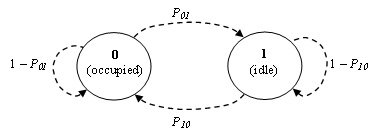
\includegraphics[width=0.7\columnwidth]{./pomdp.jpg}
				\caption{Markov channel model}
				\label{fig:pomdp}
			\end{figure}
	At the beginning of every  time slot each SU senses $M_1$ channels where $M_1 \le N$ and can access $M_2$ channels such that $M_2\le M_1$ according to the sensing results. As $M_1$ increases, the sensing time increases and the probability of finding idle channel increases, however the network throughput decreases. In addition, by increasing $M_2$, the network throughput increases, but both the energy consumption and system complexity increases. Therefore, $M_1$ and $M_2$ are design parameters affecting the performance, hardware, and energy consumption of the CR network. Since each channel is modeled as discrete-time Markov process and only a limited number of channels can be observed by SUs, spectrum access is then modeled in this paper as a POMDP model as explained in the following section. The objective of the proposed algorithm is to select the optimum value for both $M_1$ and $M_2$ based on the POMDP model. 
	
	\section{Secondary Network}
	%The objective of the proposed access strategy is to select the ${M}_{1}$ channels from the $N$ primary channels to sense and the ${M}_{2}$ channels from the ${M}_{1}$ channels to access. 
	The SU estimates the internal state of the network based on all past decisions and observations denoted by a belief vector  ${\ }{\Omega }\left({t}\right)=\left[P_1\left(t\right),P_2\left(t\right),\dots .P_N\left(t\right)\right]$where P${}_{n}(t)$ is the idle probability of channel n at the beginning of slot t. 
	It's assumed that the SUs operate with the greedy approach; this means that every SU will try to maximize its current reward without taking in consideration the effect of the current action in future reward.
	
	For time slot t if channel a is chosen and the transition probabilities ${P}_{01}$ \& ${P}_{10}$ are known, the expected reward can be calculated as follow: 
	\begin{equation}\label{9}
	r_a(t)={[p}_a\left(t\right)\left(1-P_{10}\right)+\left(1-P_a\left(t\right)P_{01}\right)]\ B_a
	\end{equation}
	
	Where ${[p}_a\left(t\right)\left(1-P_{10}\right)+\left(1-P_a\left(t\right)P_{01}\right)]\ $represents the idle probability of channel $ a $ at time slot t.
	% also the action selected for slot t is represented by
	%\begin{equation}\label{10}
	%a^*(t)=\arg\max_{a=1,2,\dots N} r^*_a(t)=\arg\max p_{ma}(t)(1-P_{10})+(1-P_a(t)P_{01})B_a
	%\end{equation}
	After a channel is selected to be detected, their belief vectors are updated according to the corresponding sensing results. Otherwise the belief vector is updated according to the markov chain. The updated belief vector is thus represented by 
	\begin{equation}\label{11}
	{\Omega }\left({t+1}\right)=\left[P_1\left(t+1\right),P_2\left(t+1\right),\dots .P_N\left(t+1\right)\right]
	\end{equation}
	
	And 
	
	\begin{equation}\label{12}
	P_n(t+1)=
	\begin{cases}
	1 & a^*=n, \Theta=1
	\\
	0 &  a^*=n, \Theta=0
	\\
	p_n(t)(1-P_{10})+(1-P_n(t)P_{01}) & a^*\neq n
	\end{cases}
	\end{equation}
	
	By using \ref{9}$\sim$\ref{12} the SU can predict the channel states and achieve maximum throughput or reward, However this all depends on that the values of transition probabilities P${}_{01}$ \& P${}_{10}$ are known to the SU which is unrealistic and so an estimation of the channel state transition probabilities by analyzing the historical data of the channel is described in the next section. Using  Maximum likelihood (ML)  technique \cite{Teodorescu2009,Craig1998}to estimate the channel state transition probabilities for a channel with $m$ states  we can conclude that
	
	\begin{equation}\label{23}
	{\hat{p}}_{ij}=\frac{n_{ij}}{\sum^m_{j=1}{n_{ij}}}
	\end{equation}
	Where ${n}_{ij}$ is the transition count for the given channel and  defined as the number of times state i is followed by state j up until the current time slot. Now If the channel has only two states (m=2), the transition probability estimation of the two state transition probabilities are given by:
	\begin{equation}\label{24}
	{\hat{p}}_{10}=\frac{n_{10}}{n_{10}+n_{11}}
	\end{equation}
	\begin{equation}\label{25}
	{\hat{p}}_{01}=\frac{n_{01}}{n_{01}+n_{00}}
	\end{equation}
	
	
	\section{Performance Under Imperfect Channel Sensing}
	So far it was assumed that the sensing errors were negligible however the performance of the secondary network depends deeply on the accuracy of the spectrum sensing used \cite{Yucek:2009:SSS:2211326.2211414} and so to be able to study the Spectrum Efficiency in the presence of sensing errors is crucial.
	At the beginning of each time slot, the sensor takes M samples of the selected channel, for simplicity the energy detector approach is used. Let $ H_0 $ and $H_1$ represent two events (hypotheses) corresponding to the cases where PUs are absent or present in the underlying spectrum, respectively. The sampled signal received at the SU, denoted as y(n), corresponding to these two hypotheses can be formulated as: 
	\begin{align}\label{kondolies}
	y(n)=\left\{\begin{matrix}
	w(n) & H_0(free)\\ 
	s(n)+w(n) & H_1 (occupied)
	\end{matrix}\right.
	\end{align}
	Where $s(n)$  denote the PU's signal with zero mean and variance $\sigma^2_{n,1}$, $ w(n) $ be the Additive White Gaussian Noise (AWGN) with zero mean and variance $\sigma^2_{n,0}$ in channel $ n $.
	
	Let $ T(y) $ denote the test statistic and $ \lambda $ be the decision threshold. The objective spectrum sensing is to make a decision on presence or absence of the PUs' signals (i.e., choose hypothesis $ H_0 $ or $ H_1 $) based on the received signals (observations). Such decision can be made by comparing the test statistic with the threshold as:
	\begin{align}\label{kondolies}
	H_0 : T(y)< \lambda
	\end{align}
	\begin{align}\label{kondolies}
	H_1 : T(y)> \lambda 
	\end{align}	
	In general there are two types of errors at the detector level the first error is when the detector senses a channel to be occupied while in fact it's free it's called False Alarm this will result of a missed opportunity to use a free spectrum.
	
	\begin{align}\label{kondolies}
	P_F= P_r (T(y)> \lambda|H_0 = 1-\Upsilon (\frac{M}{2},\frac{\lambda }{\sigma ^2_{n,0}})
	\end{align}
	
	
	The other error that may occur is when a detector decides that a channel is free while in fact it's being used by a primary user resulting in collision with the primary user or Missed Detection. The probability of false alarm probability of false alarm ${P} _ {F} $ and probability of missed detection ${P}_{MD }$are modeled as\cite{1447503} $P_MD=1-P_D $. $ P_D $ is the probability of detecting a signal on the considered frequency when it truly is present. Thus, a large detection probability is desired. It can be formulated as: 
	\begin{align}\label{kondolies}
	P_{D}= P_r (T(y)> \lambda|H_1)
	\end{align} 
	The missed detection can be formulated as: 
	\begin{align}\label{kondolies}
	P_{MD} = \Upsilon (\frac{M}{2},\frac{\lambda }{\sigma ^2_{n,0}+\sigma ^2_{n,1}})
	\end{align}	
	
	Where $\Upsilon (m,a)$ is the incomplete gamma function.
	
	
	
	\section{Simulation Results}
	In this section, the simulation results of the proposed access algorithm is discussed and compared to the Decentralized Cognitive MAC protocol (DCMAC)\cite{Zhao2007} and the random access algorithm in\cite{Lan2012}. In order to simplify the simulation, it's assumed that each channel has one pair of primary users, and operates on that particular channel and the channel bandwidth is 1 unit. Also we assume that ${M}_{1}$=${M}_{2}$=1. The simulation is done for 100 time slots with each part simulated 10000 times. Unless otherwise stated sensing errors are negligible.
	
	
	
	\section{Results}
In this section simulation results are presented to evaluate the performance of our proposed scheme with sensing errors. At the beginning of each time slot, Sus take M number of channel samples to sense with the same value of SNR. Collision to PUs occurs when Sus senses an occupied channel as idle.
Figure \ref{fig:fig1err} shows the throughput of Sus at different SNR values (0dB, 1dB and 2dB) as a function of probability of collision. The number of channels is set to N=3, number of samples take M=5, total time slots T= 30 and channel transition probabilities$ P_ {01} = 0.3 $ and $P_{11}=0.5$. As described in the figure the throughput of Sus improves as the probability of collision increases. As the portability of collision is defined as the probability of allowed collisions to occur between the SUs and PUs it will have an impact on the throughput achieved by the SUs and also on the portability of false alarm which is shown in figure \ref{fig:fig2err}. Increasing the probability of collision decreases the chances that a Sus will sense a channel to be occupied while in fact it's free and hence decreasing the false alarm probability and improving the throughput performance. on the other hand, when collision probability is at lower values, the false detection is high and thus degrading the throughput performance.
\begin{figure}
	\centering
	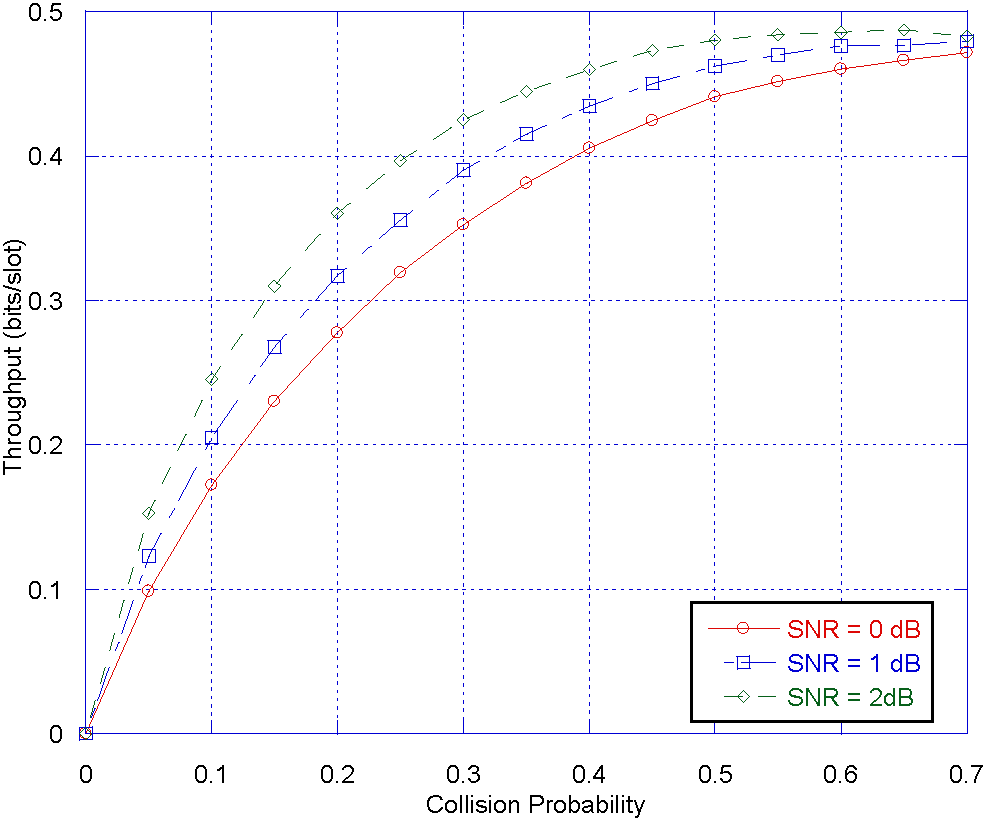
\includegraphics[width=0.5\linewidth]{./fig1_err}
	\caption{Throughput performance at different SNR values as a function of collision probability}
	\label{fig:fig1err}
\end{figure}
	\begin{figure}
		\centering
		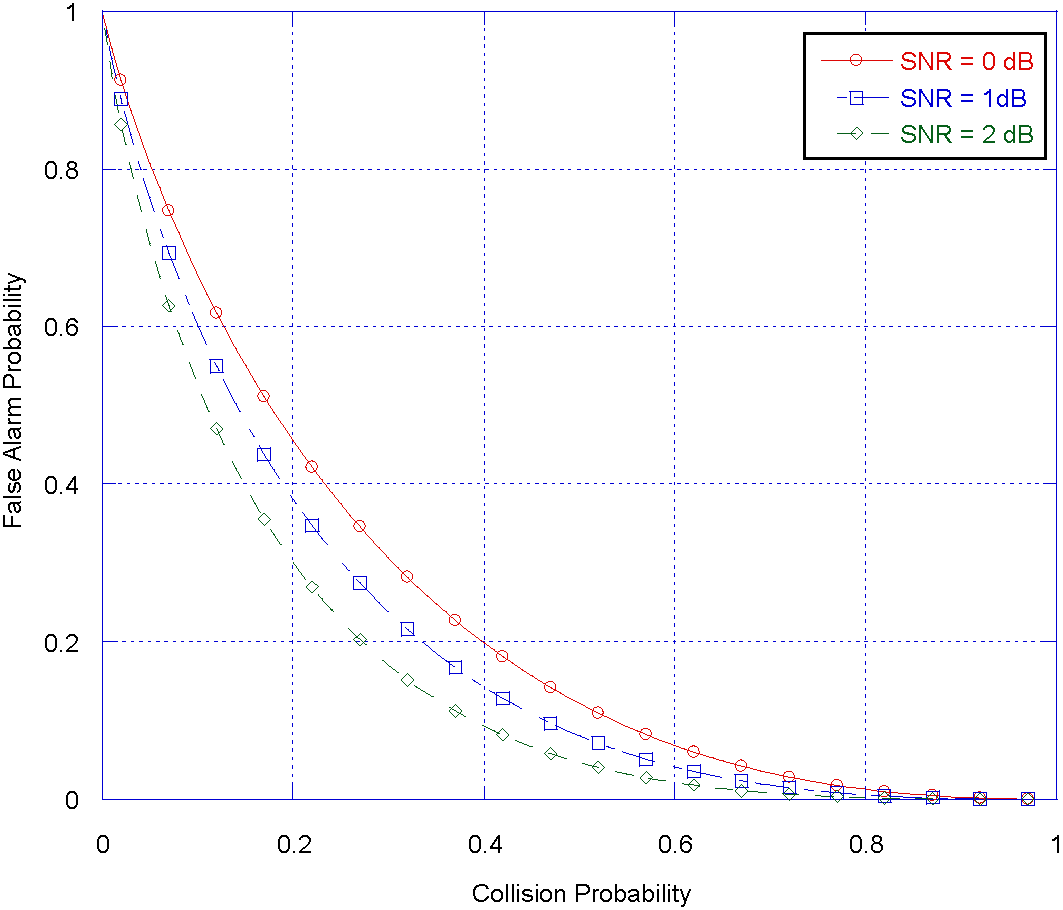
\includegraphics[width=0.5\linewidth]{./fig2_err}
		\caption{ROC curve between probability of missed detection and false alarm probability at different values of SNR }
		\label{fig:fig2err}
	\end{figure}
	. The spectrum utilization efficiency as a function of collision probability with different SNR values (0dB, 1dB and 2dB) is shown in figure \ref{fig:fig7err}. The figure shows that frequent collision can decrease the overall spectrum capacity for spectrum capacity for primary and secondary users. 


\begin{figure}
	\centering
	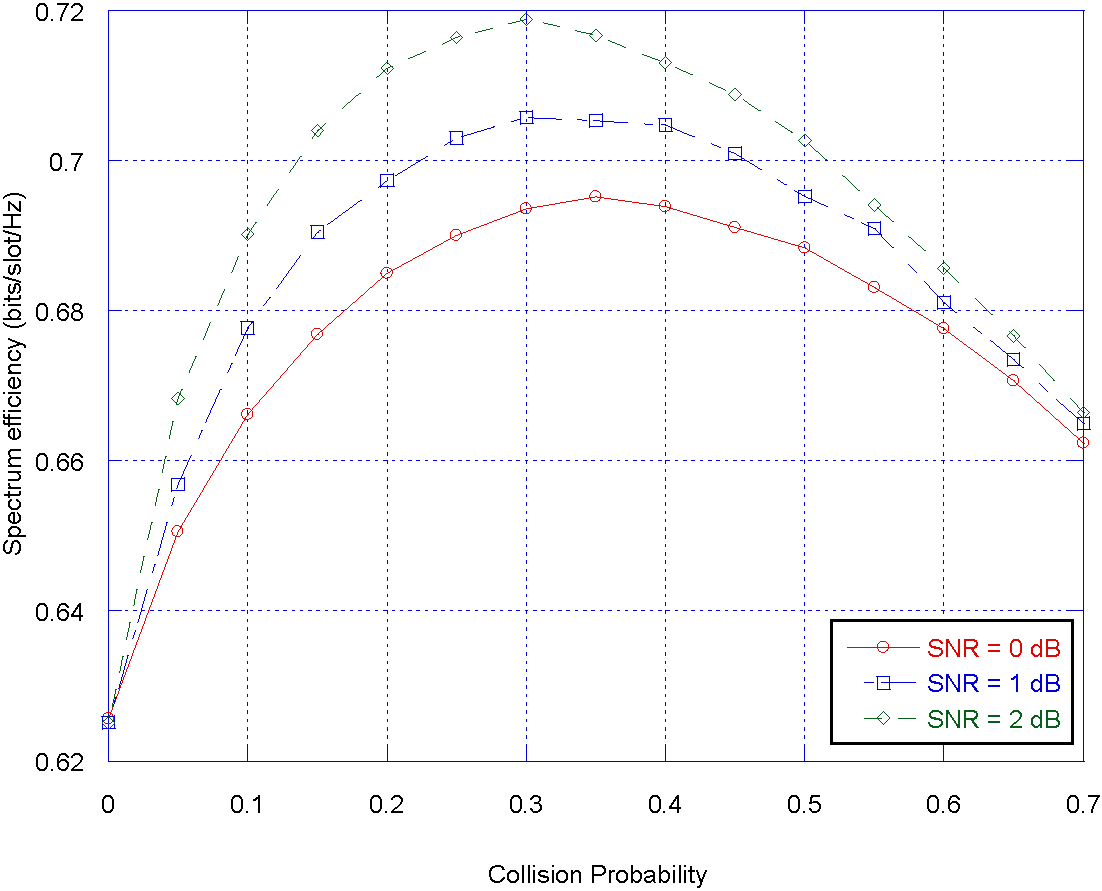
\includegraphics[width=0.5\linewidth]{./fig7_err}
	\caption{spectrum utilization efficiency as a function of collision probability}
	\label{fig:fig7err}
\end{figure}
	
%	the performance of multiple SUs with random massage arrival rate is studied in figure 6.It's assumed that the massage arrival for the SUs is a Poisson process with rate $\lambda $ and the length of the massage is determined by a geometric distribution with average of 50 packets and it takes one time slot to transmit one packet .In each time slot SUs who have no packets to transmit will go into sleep mode and will not participate in channel sensing and selection, the belief vector for these users is updated according to (12). Users who have packets to transmit will select channels according the greedy approach and update their belief vector according to the sensing outcome when more than one user selects the same channel; only one is chosen at random to transmit at that time slot. Figure 6 normalized throughput as a function of the message arrival rate $\lambda$ is shown for 5 SUs and N=3 . It's clear that as the rate of packet arrival increases the throughput of the SUs increases.
	
	
	
%	
%	\begin{figure}[h]
%		\centering{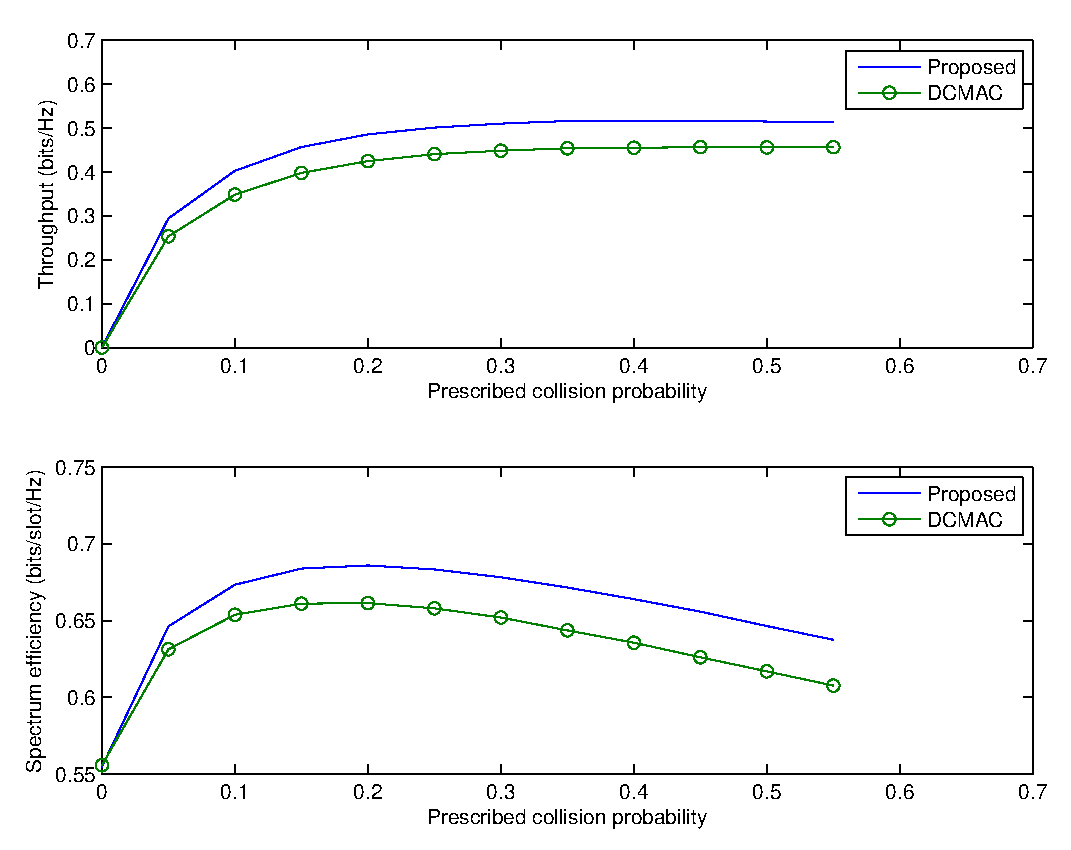
\includegraphics[width=85mm]{fig_error}}
%		\caption{Performance in the presence of imperfect sensing}
%		\label{fig4}
%	\end{figure}
	%\noindent J. Smith and A. N. Other %(\textit{The IET, Stevenage, UK})
	%\vskip3pt
	
	%\noindent E-mail: jsmith@theiet.org
	\bibliographystyle{IEEEtran}
	\bibliography{paper}
\end{document}